\documentclass[lettersize,journal]{IEEEtran}

\usepackage{amsmath,amsfonts}
\usepackage{array}
\usepackage{booktabs}
\usepackage{cite}
\usepackage{graphicx}
\usepackage{multirow}
\usepackage[caption=false,font=normalsize,labelfont=sf,textfont=sf]{subfig}
\usepackage{textcomp}
\usepackage{url}
\usepackage{xcolor}
\usepackage{xspace}
\graphicspath{{figures/}{../../experiments_mmecg/q1_paper_figures/}}

\hyphenation{op-tical net-works semi-conduc-tor radarODE radarODE-MTL REM-Net}

\newcommand{\remnet}{REM-Net\xspace}
\newcommand{\shape}{Shape-200\xspace}
\newcommand{\crrvs}{CR\_RVS\xspace}

\begin{document}

\title{\remnet: Representation--Event--Morphology Learning for Contactless ECG Beat Morphology Reconstruction from Radar}

\author{Author~Name,
        Author~Name,
        and~Author~Name%
\thanks{Author affiliations and funding information will be completed before submission.}
}

\markboth{IEEE Journal Submission Draft,~2026}%
{Author \MakeLowercase{\textit{et al.}}: \remnet\ for Contactless ECG Beat Morphology Reconstruction}

\maketitle

\begin{abstract}
Contactless electrocardiogram (ECG) reconstruction from radar could enable long-term cardiac monitoring without electrodes, yet the inverse problem remains physiologically indirect: radar observes chest-wall mechanics, whereas ECG records cardiac electrical activity. Existing studies report encouraging results, but their conclusions are difficult to compare because output targets, subject protocols, calibration assumptions, and timing metrics are often mixed. This paper studies supervised radar-to-ECG reconstruction through a morphology-first formulation. We ask whether radar supports subject-independent reconstruction of ECG beat morphology across radar modalities, and then examine why accurate morphology does not by itself imply reliable continuous ECG. We propose \remnet, a Representation--Event--Morphology network that combines a radar time-frequency representation, an auxiliary cardiac-event branch, and a morphology multi-task decoder. A temporal-alignment branch considered during model development is excluded from the final architecture because it provides no measurable morphology gain. On the public MMECG 77-GHz FMCW dataset, \remnet\ attains a \shape\ Pearson correlation coefficient (PCC) of $0.882\pm0.061$ under 11-fold strict leave-one-subject-out evaluation, exceeding an adapted radarODE-MTL baseline ($0.728\pm0.133$) on every fold (paired $p<10^{-3}$). On the public \crrvs\ 24-GHz continuous-wave dataset, it reaches $0.881\pm0.013$ under verified 5-fold subject-independent evaluation, compared with $0.550\pm0.075$ for a local baseline. The results are stable across random seeds and physiological states. An oracle assembly analysis further shows that the learned morphology can support high continuous-ECG overlap when correct beat anchors are supplied (PCC $0.93$--$0.98$), whereas predicted anchors do not generalize below 50\,ms precision. These findings indicate that, in current supervised radar-to-ECG systems, beat-anchor localization rather than morphology generation is a dominant barrier to continuous reconstruction.
\end{abstract}

\begin{IEEEkeywords}
Contactless ECG, radar sensing, FMCW radar, continuous-wave radar, ECG reconstruction, beat morphology, subject-independent evaluation.
\end{IEEEkeywords}

\section{Introduction}
\IEEEPARstart{E}{lectrocardiography} is one of the most informative tools for cardiac assessment because its PQRST morphology and temporal intervals reflect electrical depolarization and repolarization of the heart. Conventional ECG, however, depends on skin electrodes and user compliance, which limits comfort and reliability in long-term or passive monitoring scenarios. Radar sensing offers a complementary contactless route by measuring chest-wall motion caused by respiration, cardiac contraction, and other thoracic mechanical events. A reliable radar-to-ECG interface would therefore be valuable in homes, beds, vehicles, and clinical settings where continuous electrodes are inconvenient or infeasible \cite{zhang2023overview,chenmmwave,rssrnet,airecg,radarode,radarodemt}.

The technical difficulty is rooted in physiology as much as in modeling. Radar and ECG observe different domains of the same cardiac process: mechanical motion and electrical activation. Their coupling is real, but it is indirect, delayed, subject-dependent, and influenced by radar modality, posture, breathing, and signal quality. As a result, treating radar-to-ECG as a generic sequence regression problem can obscure the actual failure mode. A model may recover a plausible beat shape while placing that beat at the wrong location in a continuous trace. For cardiac monitoring, morphology, timing, and protocol are all part of the endpoint; visual waveform plausibility alone is insufficient.

The experimental landscape is similarly heterogeneous. Some studies report full-window waveform correlation, some report beat-normalized morphology, and others emphasize R-peak, PR, QRS, QT, or heart-rate metrics. Protocols range from private datasets and sample-level splits to subject-specific calibration and strict subject-independent validation. Consequently, a high reported correlation may reflect a different output target or a less stringent split rather than a better solution to the same clinical sensing problem. This distinction is especially consequential for contactless ECG, where beat morphology and continuous timing are related but not interchangeable.

We therefore take a morphology-first view of supervised radar-to-ECG reconstruction. Instead of assuming that continuous ECG recovery is already solved, we isolate a clinically meaningful and experimentally controlled subproblem: can a representation-aware, event-structured supervised model reconstruct ECG beat morphology under subject-independent protocols, and does the same principle transfer from 77-GHz FMCW radar to 24-GHz continuous-wave radar? We then use a bounded mechanism analysis to identify what prevents accurate morphology from becoming reliable continuous ECG.

We propose \remnet, a Representation--Event--Morphology network. The final model uses a cardiac-informative radar time-frequency representation, a compact encoder, an auxiliary cardiac-event branch, and a morphology multi-task decoder. An event-conditioned alignment branch was tested during development and removed after controlled ablation showed no consistent morphology gain. Thus, the final model is not presented as an alignment mechanism; it is a beat-structured supervised morphology reconstructor.

This framing leads to a different kind of contribution from simply adding another neural backbone. The central question is what radar can reconstruct reliably under subject-independent supervision. Answering it requires separating beat morphology from continuous timing, evaluating across radar modalities, and keeping calibrated, adapted, and reported-only results in distinct comparison tiers.

The main contributions are summarized as follows.
\begin{itemize}
    \item We formulate supervised radar-to-ECG as a representation--event--morphology learning problem and propose \remnet, a compact architecture that uses cardiac time-frequency representations, auxiliary event supervision, and an explicit beat-morphology decoder.
    \item We demonstrate subject-independent beat-morphology reconstruction on public MMECG, obtaining \shape\ PCC $0.882 \pm 0.061$ across 11 strict-LOSO folds, with three-seed stability of $0.885 \pm 0.002$.
    \item We validate the same supervised framework on public \crrvs\ 24-GHz CW radar, reaching PCC $0.881 \pm 0.013$ across 5 verified subject-independent folds, with three-seed stability of $0.886 \pm 0.001$.
    \item We provide an output-formulation-aware comparison protocol that separates reproduced/adapted baselines, calibrated prior results, and reported-only literature, reducing protocol-induced ambiguity in radar-to-ECG evaluation.
    \item We show, through oracle assembly and direct beat-localization measurements, that the residual continuous-ECG gap is governed by beat-anchor localization precision rather than morphology capacity alone.
\end{itemize}

\section{Related Work}

\subsection{Radar-Based Contactless Cardiac Monitoring}
Radar has become an increasingly important modality for unobtrusive physiological sensing because it can capture sub-millimeter chest-wall displacement without skin contact. Early and classical work mainly estimated respiration, heart rate, and heart-rate variability from phase modulation or spectral periodicity, while recent FMCW, UWB, and mmWave systems exploit range-time, phase, and micro-Doppler representations to recover finer cardiac motion patterns \cite{zhang2023overview,wuNonintrusiveHumanVital2024,kouhalvandi2025advances,noceraMachineLearningRADARbased2024}. This progression has moved the field from coarse vital signs toward ECG-grained cardiac monitoring. For example, UWB and mmWave systems have been used to extract cardiac-wave or ECG-like signals under controlled conditions \cite{wangECGgrainedCardiacMonitoring2022c,xuCardiacWaveMmWavebasedScheme2021,chenmmwave}. These studies establish the physiological plausibility of contactless cardiac monitoring, but they also highlight a fundamental asymmetry: radar measures mechanically expressed thoracic motion, whereas ECG records cardiac electrical activity. This electromechanical separation makes ECG reconstruction more demanding than heart-rate estimation or generic vital-sign extraction.

\subsection{Learning-Based Radar-to-ECG Reconstruction}
Deep learning has shifted radar-based ECG reconstruction from handcrafted demodulation and filtering toward data-driven mechanical-to-electrical transformation. Direct CNN, recurrent, and temporal-convolutional models learn waveform mappings from radar-derived features, whereas more recent methods introduce structure into the transformation. RSSRNet separates mixed respiratory and heartbeat components and reconstructs ECG and respiration from an STFT representation \cite{rssrnet}. radarODE and radarODE-MTL embed ODE-style priors and multi-task learning to model the domain transformation and improve robustness \cite{radarode,radarodemt}. AirECG uses cross-domain diffusion to address abnormal cardiac rhythms and subject variability \cite{airecg}, while Radar2ECG uses multi-scale fusion and semantic distillation from radar heart-sound representations \cite{radar2ecg}. Other sequence and generative approaches include ECGDiff \cite{ecgdiff}, WaveGRU-Net \cite{xu2025wavegrunet}, CUHeart \cite{li2025cuheart}, conditional diffusion from radar cardiography \cite{FromRadarCardiography}, SS-S2SA \cite{S2SA}, cross-modal autoencoders \cite{cross-modalautoencoder}, and posture-robust representation learning such as mmJEPA-ECG \cite{liu2026mmjepaecg}. For continuous-wave radar, MultiResLinkNet and BiLSTM-based models further explore reconstruction from single-channel I/Q motion signals \cite{chowdhury2024multireslinknet,g2025bilstmCW}. The diversity of these designs suggests that the problem is not merely a choice of backbone; it depends on how cardiac motion is represented, which ECG quantity is targeted, and how subject variation is controlled.

\subsection{Subject-Independent Evaluation and Output Formulation}
A recurring challenge in this literature is that model architecture, sensing hardware, output definition, and evaluation protocol are often entangled. Reported values may come from private datasets, sample-level splits, subject-specific calibration, or task formulations that are not interchangeable. VMD-CBNeT, for example, reports strong performance on the Nature/\crrvs\ source dataset \cite{xu2025vmdcbnet}, but its PCC is produced under its own ECG reconstruction protocol rather than under our beat-normalized \shape\ morphology protocol. RSSRNet and AirECG report high correlations on private or custom datasets \cite{rssrnet,airecg}, which are important evidence for the field but cannot be treated as same-protocol public-MMECG strict-LOSO comparisons. This paper therefore follows an output-formulation-aware evaluation strategy: reproduced or adapted baselines under our protocol are separated from reported-only literature, and beat morphology is explicitly distinguished from continuous ECG timing. This separation is essential for assessing whether a model improves the supervised reconstruction problem itself, rather than benefiting from a different split, target, or metric space.

\section{Method}

\subsection{Problem Formulation}
For each 8-s radar window $x$ sampled at 200 Hz and paired ECG waveform $y \in \mathbb{R}^{1600}$, the primary target is a beat-normalized morphology vector $s \in \mathbb{R}^{200}$, denoted \shape. The target is extracted from the reference center cardiac cycle, resampled to 200 points, and min--max normalized per beat. This formulation removes absolute cycle duration and amplitude scale, so that the primary endpoint is morphology fidelity rather than temporal placement. The model also predicts auxiliary cardiac-event masks, including R-peak and QRS-region masks. Full-window ECG and anchor-guided assembly are retained as diagnostic outputs for the continuous-gap analysis, not as the main reported claim.

Let $m_R \in [0,1]^{1600}$ and $m_Q \in [0,1]^{1600}$ denote soft R-peak and QRS-region targets obtained from the reference ECG. During training, these masks supervise the event branch; during final morphology evaluation, no ground-truth ECG events from the test subject are used as model inputs. The supervised mapping can therefore be written as
\begin{equation}
    (\hat{y}, \hat{s}, \hat{m}_R, \hat{m}_Q) = f_\theta(\phi(x)),
\end{equation}
where $\phi(\cdot)$ is the radar representation transform and $f_\theta$ is \remnet.

\subsection{Morphology--Anchor--Assembly Decomposition}
We use a simple decomposition to clarify why beat morphology and continuous ECG should not be treated as identical endpoints. Let a continuous ECG segment be represented as a sequence of beat morphologies $\{s_k\}_{k=1}^{K}$ placed at beat anchors $\{a_k\}_{k=1}^{K}$, where $a_k$ denotes the R-peak time or an equivalent cardiac-cycle anchor. A generic overlap-add assembly operator can be written as
\begin{equation}
    y(t) \approx \mathcal{A}(\{s_k\},\{a_k\})(t)
    = \sum_{k=1}^{K} w_k(t-a_k)\,s_k(\tau_k(t-a_k)),
    \label{eq:assembly}
\end{equation}
where $w_k$ is a local window and $\tau_k(\cdot)$ maps physical time within a beat to the normalized morphology coordinate. This expression is not meant to impose a specific clinical delineation algorithm; it formalizes the dependence of continuous ECG reconstruction on two separable quantities: the morphology assigned to each beat and the temporal anchor at which that morphology is placed.

Under this view, the continuous reconstruction error can be separated into a morphology term and an anchor term. If the assembly operator is locally Lipschitz with respect to beat shape and anchor location, then for predicted morphologies $\{\hat{s}_k\}$ and anchors $\{\hat{a}_k\}$,
\begin{equation}
\begin{split}
    \| \mathcal{A}(\{\hat{s}_k\},\{\hat{a}_k\}) -
    \mathcal{A}(\{s_k\},\{a_k\}) \| \\
    \leq C_s \sum_k \|\hat{s}_k-s_k\|
    + C_a \sum_k |\hat{a}_k-a_k|
    + \epsilon_{\mathrm{asm}},
\end{split}
\label{eq:error_decomp}
\end{equation}
where $C_s$ and $C_a$ depend on the local beat slope and windowing function, and $\epsilon_{\mathrm{asm}}$ contains residual effects such as beat overlap, amplitude normalization, and delineation error. The key implication is that a model can have a small morphology error but a large continuous error if the anchor error is comparable to the width of sharp ECG components such as the QRS complex. In that regime, improving the shape decoder alone cannot guarantee better continuous ECG.

This decomposition motivates the paper's evaluation design. The \shape\ target estimates the first term in (\ref{eq:error_decomp}) by asking whether radar contains enough information to reconstruct beat morphology under subject-independent supervision. Oracle-anchor assembly estimates the achievable continuous upper bound when the second term is removed. Predicted-anchor assembly and R-peak F1 then measure whether the learned event branch can control the second term under the same subject-independent setting. The final model is therefore evaluated primarily as a morphology reconstructor, while continuous ECG is analyzed as a morphology-plus-anchor problem.

\subsection{Radar Representation}
\remnet\ receives a cardiac-informative time-frequency representation rather than raw range-bin or I/Q samples. For MMECG, the 50 FMCW range bins are transformed into a WSST/STFT-like time-frequency representation over 8-s windows, producing a multi-bin tensor. For \crrvs, complex I/Q signals are demodulated to phase/displacement-like motion and transformed into a single-channel time-frequency representation. The two datasets therefore differ in radar modality and input-channel count, but share the same downstream modeling principle.

The representation layer has two roles. First, it reduces the likelihood that differences between methods are driven mainly by an impoverished raw input. Second, it gives FMCW range-time information and CW phase motion a common interface: both can be represented as time-frequency cardiac-motion maps. We do not present WSST/STFT itself as the novelty; it is the controlled cardiac representation on which the event and morphology learning problem is posed.

\subsection{Architecture}
Fig.~\ref{fig:overview} summarizes the architecture. The representation encoder applies lightweight multi-scale two-dimensional convolutions over the radar time-frequency map, pools over frequency, and produces a temporal latent sequence. Parallel kernels capture short cardiac transients and broader motion envelopes, while the shallow encoder keeps the model compact. The event auxiliary head predicts R-peak and QRS-region masks from the shared latent representation and projects event-aware features back into the temporal representation. The morphology decoder then reconstructs both a full 1600-sample ECG waveform and the explicit 200-point morphology head. The \shape\ head is the primary reported output.

This design mirrors the decomposition of the problem. The representation encoder tests whether radar contains cardiac-informative mechanical structure; the event branch tests whether the latent representation carries cardiac timing cues; and the morphology decoder tests whether these features can reconstruct a canonical beat shape. The network is intentionally compact. Its inductive bias comes from output structure and auxiliary supervision rather than from scale.

\begin{figure}[!t]
\centering
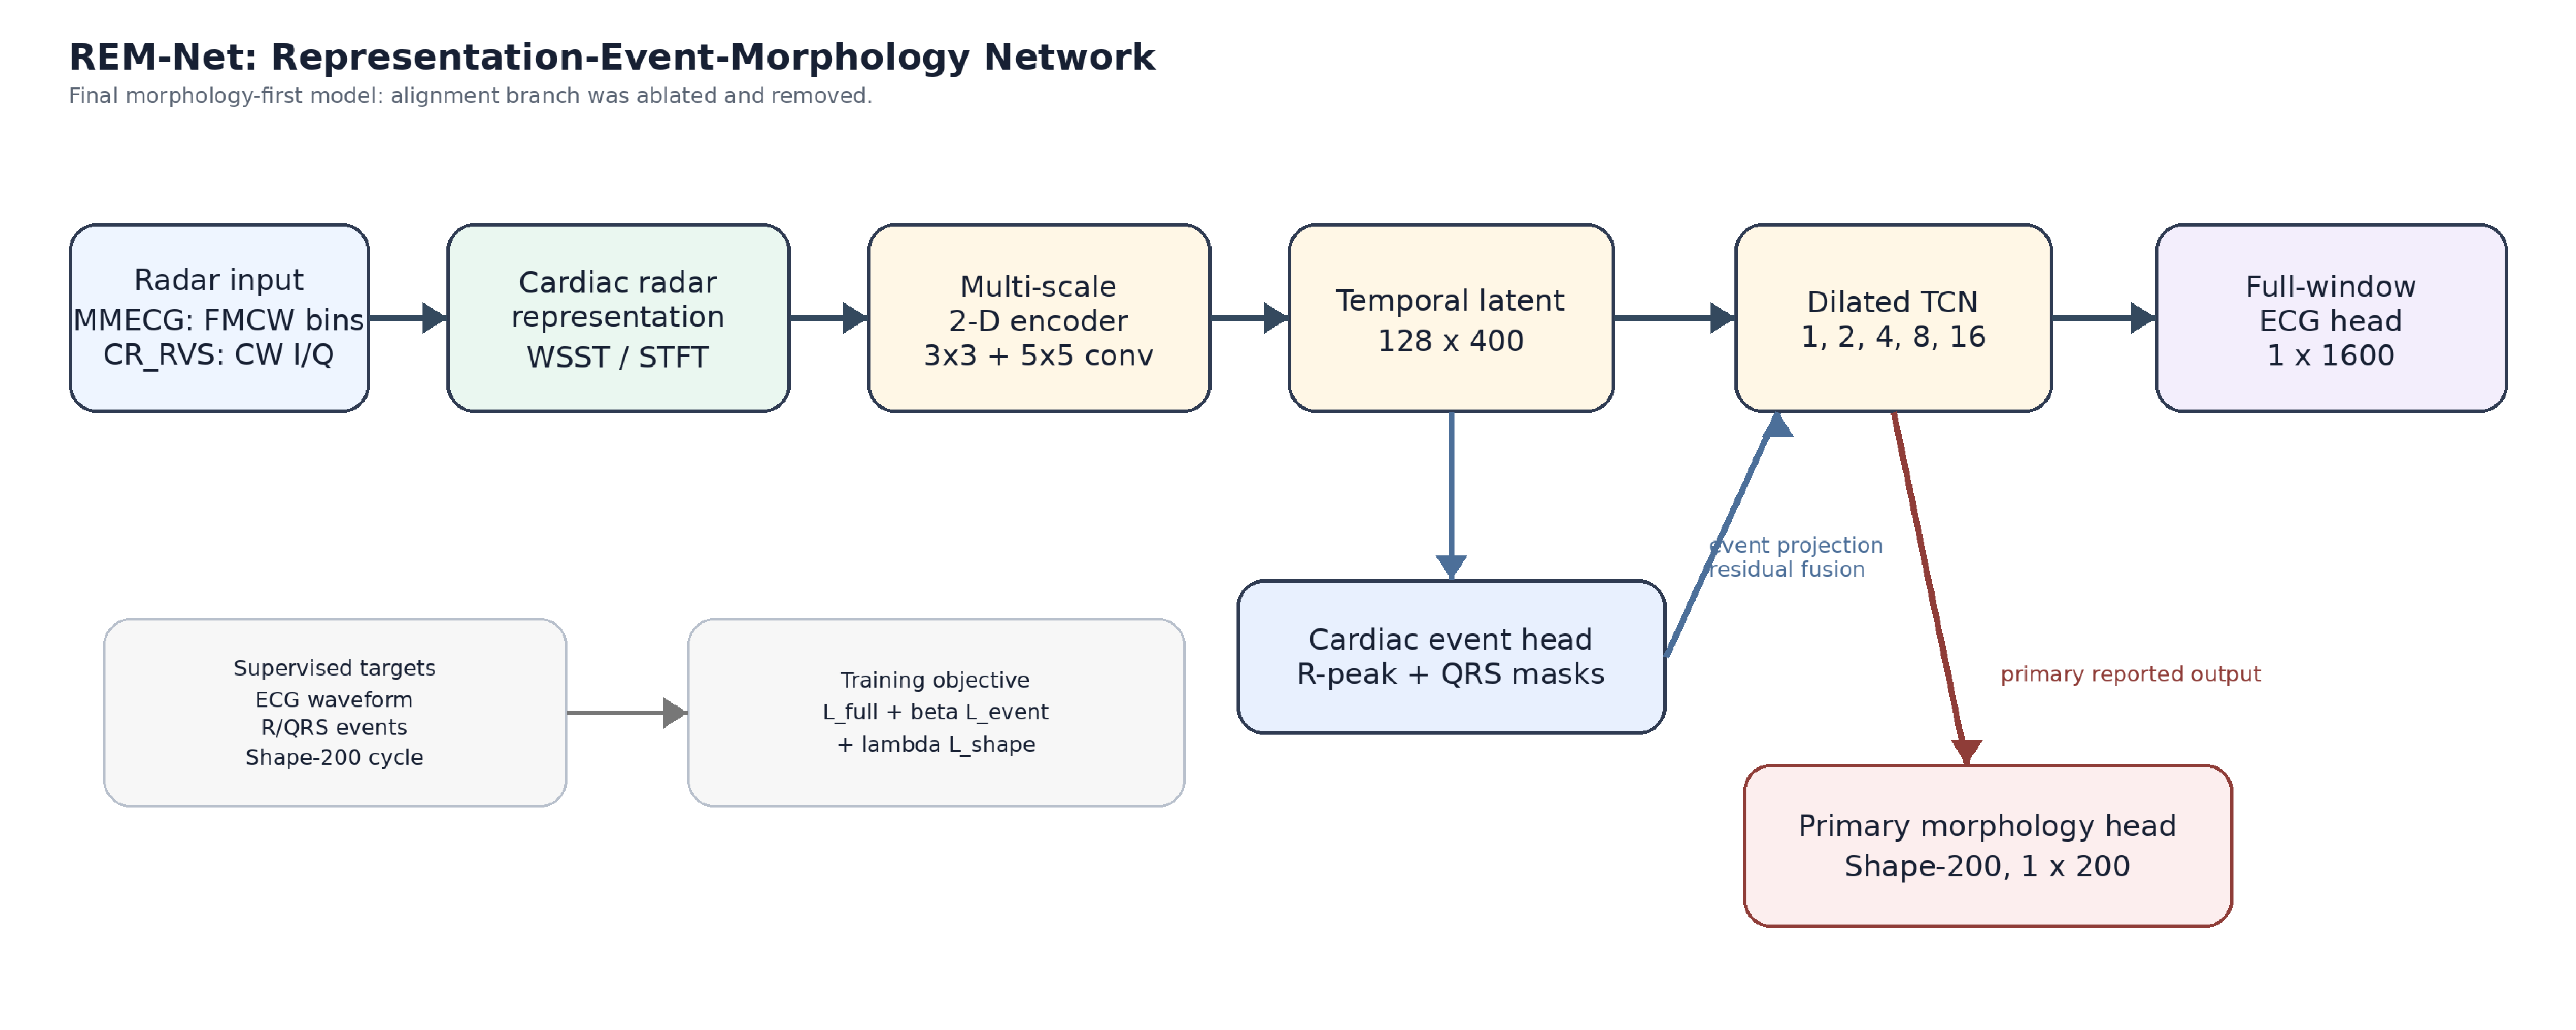
\includegraphics[width=\linewidth]{F0_remnet_overview.pdf}
\caption{Overview of \remnet. The final model uses representation encoding, event supervision, and a morphology multi-task decoder. Alignment is excluded from the final model after ablation.}
\label{fig:overview}
\end{figure}

\subsection{Representation Encoder}
The encoder first processes the radar representation through two parallel two-dimensional convolution branches with $3 \times 3$ and $5 \times 5$ kernels. Their outputs are concatenated and fused by additional convolution, normalization, nonlinear activation, dropout, and frequency pooling. The frequency dimension is then globally pooled and the temporal dimension is interpolated to 400 latent steps. A $1 \times 1$ temporal projection produces $h \in \mathbb{R}^{128 \times 400}$. This encoder is shared by MMECG and \crrvs; only the number of input channels differs.

\subsection{Cardiac Event Structure Head}
The event head upsamples $h$ to the ECG sampling grid and predicts two soft masks:
\begin{equation}
    (\hat{m}_R, \hat{m}_Q) = g_\psi(h),
\end{equation}
where $\hat{m}_R$ represents R-peak likelihood and $\hat{m}_Q$ represents a broader QRS-region likelihood. The two masks are downsampled back to the latent resolution, projected to 128 channels, and added to $h$ as a residual cardiac-structure conditioning term. This design differs from hard peak post-processing: event predictions are learned jointly and shape the latent representation during training.

\subsection{Morphology Multi-Task Decoder}
The event-conditioned latent is refined by a residual dilated TCN with dilation rates 1, 2, 4, 8, and 16. The decoder then splits into two heads. The full-window head upsamples the latent sequence to 1600 samples and predicts $\hat{y}$. The morphology head upsamples the same latent sequence to 200 samples and predicts $\hat{s}$. Both heads use one-dimensional convolutional layers with sigmoid output because the training targets are normalized. The full-window head provides auxiliary temporal supervision, while the \shape\ head is the final evaluation target.

\subsection{Training Objective}
The final supervised loss is
\begin{equation}
    \mathcal{L}
    = \mathcal{L}_{\mathrm{full}}
    + \beta \mathcal{L}_{\mathrm{event}}
    + \lambda \mathcal{L}_{\mathrm{shape}},
\end{equation}
where
\begin{equation}
    \mathcal{L}_{\mathrm{full}}
    = \| \hat{y} - y \|_1
    + \alpha \mathcal{L}_{\mathrm{MR\text{-}STFT}}(\hat{y}, y),
\end{equation}
and
\begin{equation}
    \mathcal{L}_{\mathrm{shape}}
    = \| \hat{s} - s \|_1
    + w_{\mathrm{pcc}}\left(1-\mathrm{PCC}(\hat{s},s)\right).
\end{equation}
The event loss is binary cross entropy between predicted and reference event masks. The final configuration is $\alpha=0.1$, $\beta=0.3$, $\lambda=0.8$, and $w_{\mathrm{pcc}}=0.5$. Models are trained fold-wise with AdamW and validation-only checkpoint selection.

The full-window term stabilizes low-level waveform learning and spectral smoothness, whereas the \shape\ term directly optimizes the primary morphology target. The event term is not used to claim clinical event detection; it regularizes the latent space toward cardiac structure and later provides a diagnostic handle for the continuous-gap analysis. The loss is fixed for all final runs to avoid post-hoc metric tuning.

\subsection{Removed Alignment Module}
An earlier model variant included an event-conditioned temporal-alignment branch motivated by the electromechanical gap between radar motion and ECG electrical activation. In controlled morphology ablation, however, this branch changed \shape\ PCC only within approximately $\pm 0.005$, with inconsistent sign across folds. We therefore remove it from the final model and keep continuous alignment as a separate mechanism analysis. This design choice is deliberate: the final claim is not an alignment-based continuous-ECG model, but a morphology model accurate enough to expose where the continuous gap remains.

\subsection{Implementation Details}
Unless otherwise stated, \remnet\ uses 128 hidden channels, a dilated temporal convolutional decoder, min--max normalized \shape\ targets, and validation-best checkpoint selection. Training uses AdamW with learning rate $10^{-4}$, weight decay $10^{-4}$, batch size 16, and early stopping. MMECG uses the narrow-band cardiac preprocessing selected before final evaluation; \crrvs\ uses the CW phase/displacement representation without narrow-band filtering. The final model contains approximately 1.79M parameters. All reported final-test numbers are produced from held-out folds after the architecture and hyperparameters have been fixed.

\section{Experimental Setup}

\subsection{Datasets}
MMECG is a public 77-GHz FMCW radar dataset with time-aligned ECG. We use 8-s, 200-Hz windows and 11-fold strict leave-one-subject-out evaluation. The held-out subject never contributes to training, normalization, range-bin selection, or checkpoint selection.

\crrvs\ is a public 24-GHz continuous-wave radar dataset with I/Q radar and Lead-II ECG across 30 subjects and multiple physiological states. We use a verified 5-fold subject-independent split with no train--test subject overlap and no subject appearing in more than one test fold. The 30 subjects are partitioned into test folds of size 7/7/7/5/4.

\subsection{Leakage Control and Checkpoint Policy}
Because radar-to-ECG datasets are small, leakage control is as important as model design. All preprocessing statistics used by the model are computed without the held-out test subject. Test-subject ECG is used only for supervised target construction during evaluation and never for range-bin selection, normalization fitting, checkpoint selection, or threshold tuning of a final model. Oracle analyses that use ground-truth anchors are labeled as upper bounds and excluded from the main model comparison.

For each fold, checkpoints are selected using validation performance only. The seed-42 run is used as the pre-specified final-test row, while the three-seed run is reported as a stability analysis. This distinction separates subject variability, measured by fold-level standard deviation, from training stochasticity, measured by across-seed standard deviation.

\subsection{Metrics and Aggregation}
The primary metric is \shape\ PCC. We also report RMSE, MAE, and $R^2$ in the \shape\ normalization space, plus region-wise morphology PCC over QRS-edge, ST/T, and diastolic regions. Per-segment metrics are averaged within each fold and then reported as fold-macro mean and standard deviation. Main \remnet\ rows report the pre-specified final-test seed-42 run, and three-seed statistics are used to verify training stability. NeuroKit2 is used where ECG delineation is required for auxiliary analysis \cite{neurokit2}.

Region-wise morphology metrics are included to prevent a single global PCC from overstating clinical shape fidelity. The QRS-edge region evaluates sharp depolarization morphology, the ST/T region evaluates repolarization-related morphology, and the diastolic region measures the low-amplitude interval where radar signal-to-noise is weakest. These regions are fixed by normalized beat phase rather than selected post hoc.

\subsection{Baseline and Literature Tiers}
Table~\ref{tab:tiers} defines the comparison policy. Only proposed and adapted/local baselines under our subject-independent morphology protocol enter the main fair-comparison blocks. Reported-only literature is included for context but not merged into the same-protocol ranking.

The adapted radarODE-MTL baseline is evaluated only in morphology/ECG\_shape space, which is the closest comparable output to \shape. We do not claim to reproduce its official long-term assembly. The available BeatAware result is reported separately because it uses target-subject calibration and different preprocessing. These distinctions reduce the apparent size of the headline table, but they avoid a more serious problem: comparing numbers that answer different experimental questions.

\begin{table}[!t]
\centering
\caption{Comparison Tiers Used in This Paper}
\label{tab:tiers}
\begin{tabular}{p{0.18\linewidth}p{0.70\linewidth}}
\toprule
Tier & Meaning \\
\midrule
Proposed & \remnet\ under our predefined subject-independent protocol. \\
Adapted & Baseline implemented or adapted under our protocol; protocol differences are stated. \\
Calibration prior & Historical result using target-subject calibration; separated from strict subject-independent rows. \\
Reported-only & Published number from another paper, not reproduced under our protocol; never used as same-protocol evidence. \\
\bottomrule
\end{tabular}
\end{table}

\section{Results}

\subsection{MMECG Beat-Morphology Reconstruction}
Table~\ref{tab:mmecg} reports MMECG \shape\ results under strict 11-fold LOSO. \remnet\ gives the highest morphology reconstruction accuracy, with final-test PCC $0.882 \pm 0.061$ and three-seed stability $0.885 \pm 0.002$. The strongest adapted baseline is radarODE-MTL in its ECG\_shape/morphology space, with PCC $0.728 \pm 0.133$. REM-Event and WSST-TCN remain far lower, indicating that the final result is not explained by the time-frequency representation alone.

The comparison with radarODE-MTL is informative because radarODE-MTL is a structured baseline rather than a weak generic regressor. Its adapted morphology result suggests that dynamic or multi-task formulations alone do not guarantee high beat-shape fidelity under the strict LOSO \shape\ protocol. Conversely, the low WSST-TCN result shows that the representation layer by itself is insufficient. The empirical gain comes from the combination of cardiac representation, event-structured supervision, and a morphology-specific decoder.

The improvement over radarODE-MTL is consistent and statistically significant. \remnet\ achieves a higher per-fold \shape\ PCC on all 11 held-out subjects (mean difference $+0.154$; paired $t$-test $p=9.8\times10^{-5}$, Wilcoxon signed-rank $p=9.8\times10^{-4}$). The margin is in fact largest on the two hardest subjects (folds~5 and~9), where \remnet\ reaches $\approx0.76$ against $\approx0.48$ for radarODE-MTL, indicating that the advantage is not driven by easy subjects.

\begin{table}[!t]
\centering
\caption{MMECG \shape\ Morphology Reconstruction under 11-Fold Strict LOSO. Comparators
are restricted to methods that produce a credible morphology result under our common
protocol. Baselines whose public code was designed for a different dataset/output space
(e.g., RSSRNet, AirECG) are not forced into this table; their original reported numbers
are quoted as different-dataset context in Table~\ref{tab:reported}.}
\label{tab:mmecg}
\begin{tabular}{llccc}
\toprule
Method & Tier & PCC & RMSE & MAE \\
\midrule
\remnet & Proposed & $\mathbf{0.882 \pm 0.061}$ & 0.112 & 0.090 \\
radarODE-MTL & Adapted & $0.728 \pm 0.133$ & 0.139 & 0.106 \\
REM-Event & Ablation & $0.279 \pm 0.151$ & 0.258 & 0.183 \\
WSST-TCN & Representation & $0.273 \pm 0.151$ & 0.258 & 0.183 \\
\midrule
BeatAware & Calibration prior$^\dagger$ & $0.671 \pm 0.159$ & 0.195 & 0.145 \\
\bottomrule
\end{tabular}

\vspace{2pt}
\footnotesize $^\dagger$BeatAware uses LOSO with target-subject calibration and is
therefore not a strict subject-independent comparator; it is shown for reference only.
\end{table}

\subsubsection{Per-subject spread}
Because subject-independent averages can hide worst-case behaviour, we report the
per-fold spread of the final-test run rather than only the mean. On MMECG, the
per-fold \shape\ PCC ranges from 0.756 (fold~5) to 0.947 (fold~4); two held-out subjects
(folds~5 and~9) are noticeably harder at $\approx$0.76, while the remaining nine folds lie
between 0.858 and 0.947. This subject variability is the source of the $\pm0.061$
across-fold standard deviation and is consistent with lower-SNR recordings for those
subjects. On \crrvs, per-fold PCC is far more uniform (0.867--0.903, $\pm0.013$),
indicating that the CW morphology result is not driven by a single easy subject. We
report these ranges explicitly so that the aggregate numbers are not read as uniform
across subjects.

\subsection{Morphology Is Not Only a Global PCC Effect}
Table~\ref{tab:regions} reports region-wise morphology PCC. On MMECG, \remnet\ and radarODE-MTL are both accurate near the QRS edge, but radarODE-MTL loses fidelity in ST/T and diastolic regions. \remnet\ preserves broader morphology, reaching ST/T PCC 0.787. On \crrvs, \remnet\ improves QRS-edge morphology over CW-STFT+TCN and remains competitive in ST/T, while diastolic morphology remains the weakest region.

This analysis is included because beat-normalized PCC can reward smooth, average-looking curves. The QRS-edge result shows that \remnet\ retains the sharp part of the beat, while the ST/T result indicates that the model is not merely detecting the dominant R/QRS deflection. The diastolic weakness is also informative: this region has lower amplitude and weaker radar coupling, particularly in CW radar, and remains a limitation for clinically complete morphology recovery.

\begin{table}[!t]
\centering
\caption{Region-Wise Morphology PCC}
\label{tab:regions}
\begin{tabular}{llccc}
\toprule
Dataset & Method & QRS-edge & ST/T & Diastolic \\
\midrule
MMECG & \remnet & 0.962 & 0.787 & 0.510 \\
MMECG & radarODE-MTL & 0.961 & 0.157 & 0.034 \\
\crrvs & \remnet & 0.941 & 0.793 & 0.380 \\
\crrvs & CW-STFT+TCN & 0.464 & 0.744 & 0.358 \\
\bottomrule
\end{tabular}
\end{table}

\begin{figure}[!t]
\centering
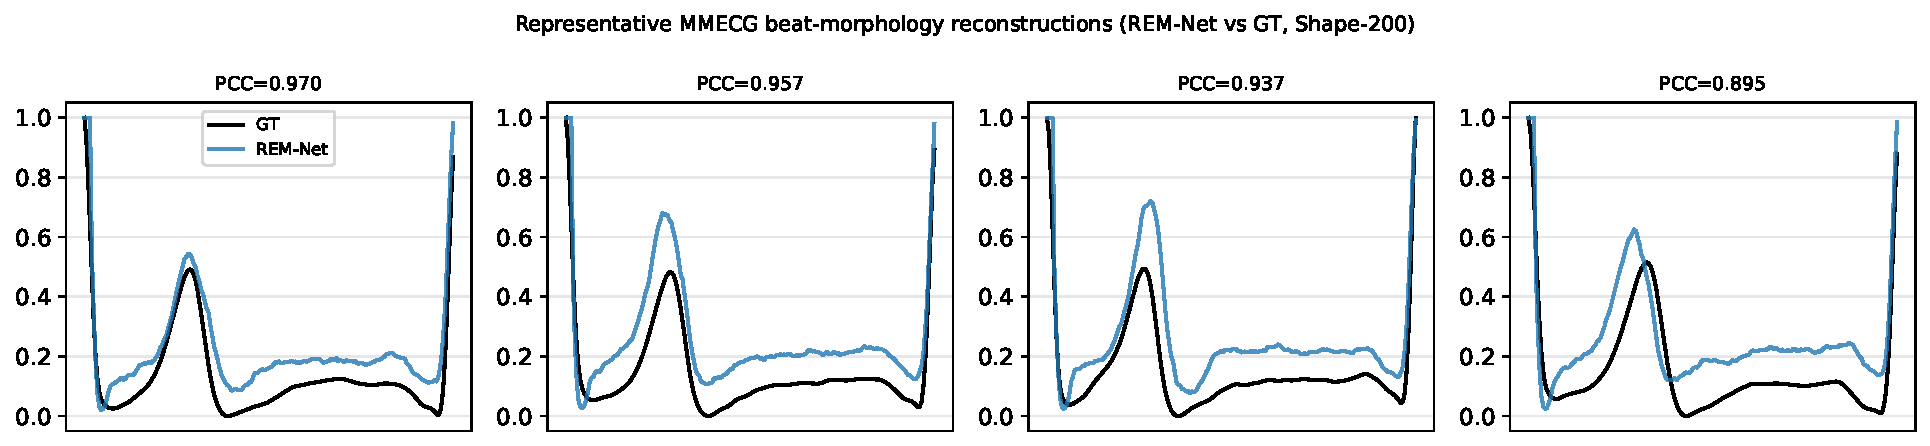
\includegraphics[width=\linewidth]{F5_morphology_examples.pdf}
\caption{Representative beat-morphology reconstructions selected by a deterministic high/median/hard rule. The purpose of this figure is not to hand pick visually perfect examples, but to show the typical morphology agreement and failure modes behind the aggregate \shape\ PCC.}
\label{fig:qualitative}
\end{figure}

\subsection{Physiological-State Breakdown}
Table~\ref{tab:states} reports \shape\ PCC broken down by the physiological state
recorded in each dataset (normal breathing, irregular breathing, breath-hold/sustained
respiration, and post-exercise). Morphology reconstruction is comparatively stable under respiratory
perturbation on both datasets: PCC drops only from 0.912 to 0.903 (MMECG) and from 0.887
to 0.877 (\crrvs) between normal and irregular breathing. The largest degradation is under
post-exercise on MMECG (0.834), where elevated heart rate and residual body motion reduce
the radar signal-to-noise ratio. We report this breakdown because aggregate morphology
scores can hide state-dependent behaviour that a monitoring system would encounter in
practice; the gradual degradation is consistent with the morphology-first model remaining usable under several physiological conditions.

\begin{table}[!t]
\centering
\caption{\shape\ PCC by Physiological State}
\label{tab:states}
\begin{tabular}{lcc}
\toprule
Physiological state & MMECG & \crrvs \\
\midrule
Normal breathing & 0.912 & 0.887 \\
Irregular breathing & 0.903 & 0.877 \\
Breath-hold / sustained & 0.850 & 0.869 \\
Post-exercise & 0.834 & --- \\
\bottomrule
\end{tabular}
\end{table}

\subsection{Robustness to Input Noise}
We further stress-test the final model by injecting additive Gaussian noise into its time-frequency input. The noise standard deviation is set to a multiple of each window's representation standard deviation, so the multiplier is an inverse signal-to-noise ratio (level $1.0$ corresponds to $0$\,dB). This is a controlled input-corruption test, not a motion-artifact simulation. Table~\ref{tab:noise} reports the resulting \shape\ PCC. On MMECG, performance changes modestly up to noise equal to the input amplitude ($0.834$ at $0$\,dB, a $5.4\%$ relative drop) and remains usable at $-6$\,dB ($0.781$). The \crrvs\ dataset degrades more rapidly at every level ($-12\%$ vs $-2.5\%$ at $+6$\,dB). This difference is consistent with modality redundancy: MMECG provides 50 range bins whose information the model can average over, whereas \crrvs\ is single-channel continuous-wave with no comparable spatial redundancy. The contrast reinforces why cross-modality validation is necessary.

\begin{table}[!t]
\centering
\caption{\shape\ PCC under additive input noise for the final model (fold-macro mean $\pm$ std). Level is the ratio of noise std to input std ($\approx$ inverse SNR); level $0$ is the clean final-test number.}
\label{tab:noise}
\begin{tabular}{lcc}
\toprule
Noise level ($\approx$SNR) & MMECG (FMCW) & \crrvs\ (CW) \\
\midrule
0.0 (clean)   & $0.882 \pm 0.061$ & $0.881 \pm 0.013$ \\
0.5 ($+6$\,dB) & $0.860 \pm 0.073$ & $0.775 \pm 0.087$ \\
1.0 ($0$\,dB)  & $0.834 \pm 0.112$ & $0.602 \pm 0.223$ \\
2.0 ($-6$\,dB) & $0.781 \pm 0.123$ & $0.418 \pm 0.298$ \\
3.0 ($-9.5$\,dB) & $0.646 \pm 0.150$ & $0.257 \pm 0.316$ \\
5.0 ($-14$\,dB) & $0.390 \pm 0.215$ & $0.129 \pm 0.268$ \\
\bottomrule
\end{tabular}
\end{table}

\subsection{External Validation on \crrvs}
Table~\ref{tab:crrvs} reports \crrvs\ external validation. Under verified 5-fold subject-independent evaluation, \remnet\ reaches \shape\ PCC $0.881 \pm 0.013$ in the pre-specified final-test run and $0.886 \pm 0.001$ across three seeds. This is substantially higher than the local CW-STFT+TCN baseline. The VMD-CBNeT and CNN+LSTM values are shown as reported-only context from the same source dataset, but their protocol and PCC space differ from ours.

The \crrvs\ experiment changes more than the data source. It changes the radar physics from multi-bin 77-GHz FMCW to single-channel 24-GHz CW I/Q phase motion. Maintaining high morphology fidelity in this setting suggests that the formulation is not tied to one radar front end. At the same time, the table is deliberately split into local and reported-only blocks. This prevents the external validation from becoming an unfair numerical contest against methods evaluated under different segmentation, normalization, and output definitions.

\begin{table}[!t]
\centering
\caption{\crrvs\ External Validation}
\label{tab:crrvs}
\begin{tabular}{llcc}
\toprule
Block & Method & PCC & RMSE \\
\midrule
A: local protocol & \remnet & $\mathbf{0.881 \pm 0.013}$ & 0.108 \\
A: local protocol & CW-STFT+TCN & $0.550 \pm 0.075$ & 0.174 \\
\midrule
B: reported-only & VMD-CBNeT \cite{xu2025vmdcbnet} & 0.856 & 0.112 \\
B: reported-only & CNN+LSTM \cite{xu2025vmdcbnet} & 0.647 & 0.127 \\
\bottomrule
\end{tabular}
\end{table}

\subsection{Ablation and Efficiency}
The main ablation chain is WSST-TCN $\rightarrow$ REM-Event $\rightarrow$ \remnet. PCC increases from 0.273 to 0.279 with the event-only branch and then to 0.882 with the morphology multi-task decoder. Thus, the event branch alone is not sufficient; it becomes useful when paired with an output formulation that explicitly asks the network to reconstruct beat morphology. The removed alignment module has no measurable morphology benefit.

Table~\ref{tab:efficiency} contrasts model size against morphology accuracy. \remnet\ attains the highest \shape\ PCC with only $1.79$M parameters---about $15\times$ smaller than the radarODE-MTL morphology comparator ($26.8$M) yet more accurate ($0.882$ vs $0.728$), and about $2.7\times$ smaller than the BeatAware calibration-prior model. This supports the interpretation that the gain comes from output structure and auxiliary supervision rather than parameter count. Single-window inference takes $0.98$\,ms on an RTX 4080 SUPER (batch size 1), which is compatible with real-time use.

\begin{table}[!t]
\centering
\caption{Model efficiency versus morphology accuracy. Parameter counts are exact; latency is measured for the deployed model only (single 8-s window, batch size 1, RTX 4080 SUPER). $^{\dagger}$BeatAware is a calibration-prior result (Block B), not a strict-LOSO comparable number.}
\label{tab:efficiency}
\begin{tabular}{lccc}
\toprule
Model & Params & Latency & \shape\ PCC \\
\midrule
\remnet\ (ours)   & $\mathbf{1.79}$M & $0.98$\,ms & $\mathbf{0.882}$ \\
WSST-TCN          & $1.47$M & --- & $0.273$ \\
radarODE-MTL      & $26.8$M & --- & $0.728$ \\
BeatAware & $4.85$M & --- & $0.671^{\dagger}$ \\
\bottomrule
\end{tabular}
\end{table}

The ablation also clarifies how the model should be interpreted. Event supervision is not sufficient on its own; it becomes useful when the output formulation gives the network a morphology target that can exploit the event-structured latent. This is why the final model is named Representation--Event--Morphology rather than Representation--Alignment or simply WSST-TCN.

\subsection{Reported Literature Context}
Table~\ref{tab:reported} summarizes representative reported-only literature. These rows are not used as same-protocol evidence. They help position the field and clarify which published results share a source dataset, which use different protocols, and which are private-dataset context.

\begin{table*}[!t]
\centering
\caption{Reported Literature Context. Values Are Reported-Only Unless Marked as Adapted in Our Tables}
\label{tab:reported}
\begin{tabular}{llllp{0.31\linewidth}}
\toprule
Paper & Method & Dataset relation & Protocol status & Reported result / role \\
\midrule
VMD-CBNeT \cite{xu2025vmdcbnet} & VMD-CBNeT & Same source \crrvs & Different protocol & PCC 0.856, RMSE 0.112; contextual reference, not same-protocol comparison. \\
MultiResLinkNet \cite{chowdhury2024multireslinknet} & 1-D CNN & Same source \crrvs & Different metric space & Reports temporal/spectral correlation on Resting/Valsalva/Apnea segments. \\
LifWavNet \cite{lifwavnet} & Lifting wavelet net & Same source \crrvs & Different split/target & Reports CR\_RVS waveform metrics; candidate for future reproduction. \\
Radar2ECG \cite{radar2ecg} & Semantic distillation & Same source subset & Resting/sample split & Radar heart-sound to ECG generation; not our subject-independent morphology protocol. \\
RSSRNet \cite{rssrnet} & RSSRNet & Different dataset & Private/custom & Reports median ECG PCC $\approx$0.96 on its own mmWave dataset; different dataset, not numerically comparable to our protocol. \\
AirECG \cite{airecg} & Diffusion & Different dataset & Private/custom & Reports PCC $\approx$0.96 (normal)/0.86 (abnormal) on its own arrhythmia dataset; context only, not numerically comparable. \\
\bottomrule
\end{tabular}
\end{table*}

\subsection{Mechanistic Analysis of the Continuous Gap}
The high \shape performance of \remnet should not be read as evidence of reliable continuous ECG reconstruction. With ground-truth beat anchors used only for oracle analysis, the learned morphology assembles into near-perfect continuous ECG with PCC 0.93--0.98. Predicted-anchor assembly, however, collapses on harder held-out subjects. Threshold tuning can recover coarse detection recall, but continuous overlap-add does not recover because anchor localization precision does not generalize at the sub-50 ms level. Matched-beat error is approximately 16--20 ms on the easy fold but 40--55 ms on harder folds. The continuous gap is therefore governed by beat-anchor localization precision rather than morphology-generation capacity alone.
This observation is consistent with the decomposition in (\ref{eq:error_decomp}): once morphology error is small, the anchor term becomes the dominant contributor to continuous waveform mismatch, especially around the high-slope QRS region.

\subsubsection{Predicted-anchor localization is tolerance-limited}
To quantify predicted-anchor precision directly, we evaluate the final model's auxiliary event head (R-peak mask) against reference R-peaks, matched one-to-one within a tolerance window (Table~\ref{tab:rate}). On MMECG, beats are detected reliably at a coarse tolerance (F1 $0.806$ at 150 ms) but detection degrades sharply as the tolerance tightens ($0.749$ at 100 ms; $0.544$ at 50 ms). Heart rate is nonetheless recovered almost exactly ($0.32$ bpm error) because zero-mean beat-to-beat jitter averages out over a window; the deficit is fine-grained placement, not gross rate. The same event head applied to CW \crrvs\ largely fails to localize beats under subject-independent evaluation (F1 $\approx 0.10$ at all tolerances), even though the same model reconstructs \crrvs\ morphology at PCC $0.881$. This dissociation---transferable morphology but non-transferable beat localization, markedly worse on CW---is the main empirical evidence that the continuous barrier is anchor localization precision rather than morphology.

\begin{table}[!t]
\centering
\caption{Beat-localization metrics from the final \remnet\ event head (predicted anchors), fold-macro mean $\pm$ std. F1 is reported at three matching tolerances; RR and HR are conditional on matched beats. MMECG RR/HR cover $92.8\%$ of windows; \crrvs\ RR/HR are omitted because only $4.2\%$ of windows contain matched beats.}
\label{tab:rate}
\begin{tabular}{lcc}
\toprule
Metric & MMECG (FMCW) & \crrvs\ (CW) \\
\midrule
R-peak F1 @ 50\,ms $\uparrow$  & $0.544 \pm 0.153$ & $0.084 \pm 0.017$ \\
R-peak F1 @ 100\,ms $\uparrow$ & $0.749 \pm 0.127$ & $0.099 \pm 0.018$ \\
R-peak F1 @ 150\,ms $\uparrow$ & $0.806 \pm 0.083$ & $0.102 \pm 0.019$ \\
RR error (ms) $\downarrow$     & $30.4 \pm 5.7$    & --- \\
HR error (bpm) $\downarrow$    & $0.32 \pm 0.06$   & --- \\
\bottomrule
\end{tabular}
\end{table}

This result is negative for continuous reconstruction but useful scientifically. It rules out the simplest explanation that the learned morphology is too poor to form continuous ECG. If correct anchors are provided, the same morphology is sufficient for high continuous assembly. It also rules out a pure recall explanation: lowering the detection threshold recovers many missed beats but introduces false positives and does not restore overlap-add PCC. The remaining bottleneck is precision of beat placement under unseen-subject radar variability. This is more actionable than simply reporting that full-window PCC is low.

\begin{figure}[!t]
\centering
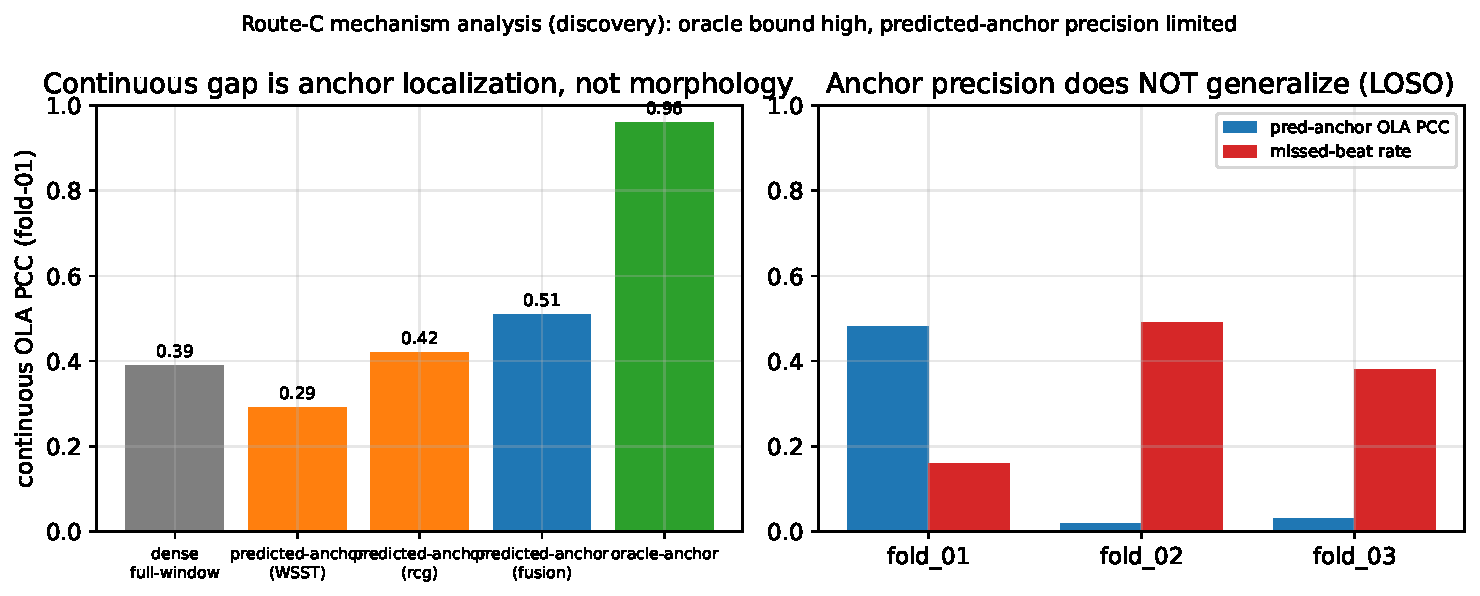
\includegraphics[width=\linewidth]{F4_route_c_mechanism.pdf}
\caption{Mechanistic analysis of the continuous gap. Oracle anchors reveal a high morphology-to-continuous upper bound, whereas predicted anchors fail to generalize with sub-50 ms precision.}
\label{fig:continuous_gap}
\end{figure}

\section{Discussion}
\subsection{What the Results Support}
The evidence supports a morphology-first claim: \remnet\ reconstructs ECG beat morphology across FMCW and CW radar under subject-independent protocols. The result is stable across seeds, transfers across radar modality, and improves over adapted/local baselines in the same morphology space. Region-wise analysis further shows that the gain is not only a smooth normalized PCC effect; \remnet\ preserves ST/T morphology where a strong adapted ODE baseline is weak. The morphology remains usable across physiological states and degrades gradually under input noise---on FMCW it changes only modestly up to $0$\,dB input noise---and it is obtained with a compact model ($1.79$M parameters, sub-millisecond inference) that is an order of magnitude smaller than the structured morphology comparator yet more accurate. The faster degradation on single-channel CW than on multi-bin FMCW is consistent with the redundancy of the sensing modality.

The main advance is therefore not an isolated architectural component. It is a reformulation of supervised radar-to-ECG as a morphology-first, output-aware evaluation problem with controlled evidence. The model is compact, the final alignment branch is removed, and the comparison table separates what is reproduced under our protocol from what is only reported in prior work. This makes the contribution narrower than an end-to-end continuous-ECG claim, but also more defensible.

\subsection{What the Results Do Not Support}
The results do not prove continuous long-term ECG recovery. \shape\ is a beat-normalized target, and continuous ECG requires accurate placement of each beat on the time axis. The oracle-anchor analysis shows that morphology is sufficient for high assembly if beat anchors are correct, but predicted anchors do not generalize at the necessary precision. Direct beat-localization measurements corroborate this: the event head detects beats at coarse tolerance ($0.806$ F1 at $150$\,ms on MMECG) but performs much worse at $50$\,ms ($0.544$), and on CW radar it largely fails to localize beats ($\approx 0.10$ F1) even though morphology remains high. Continuous radar-to-ECG should therefore be framed as an open timing-localization problem rather than a completed waveform-regression task.

This boundary is especially important when comparing with papers that report full-window ECG or clinical interval errors. Our morphology results should not be used to claim superior PR, QRS, QT, or QTc interval estimation. They also should not be used to claim that \remnet\ reproduces radarODE-MTL long-term assembly or VMD-CBNeT's original protocol. The paper's defensible position is narrower: morphology is accurate and transferable; continuous timing remains open; the mechanism analysis explains why.

\subsection{Implications for Radar-to-ECG Evaluation}
The practical implication is that future radar-to-ECG studies should report the output formulation explicitly. A method that reconstructs beat morphology, a method that reconstructs an 8-s ECG window, and a method that estimates ECG intervals are solving related but non-identical tasks. A single ranking table without protocol tiers can obscure rather than clarify progress.

\section{Limitations}
The main limitation is output formulation. \shape\ morphology is not equivalent to continuous clinical ECG. Our full-window interval-timing errors are not better than the strongest reported interval results under different protocols, and we do not claim better PR/QRS/QT interval estimation. VMD-CBNeT is reported as a contextual reference, not an identical-protocol reproduction. radarODE-MTL is compared only in morphology/ECG\_shape space; its official long-term assembly is not reproduced. Some adapted low-scoring baselines have incomplete historical preprocessing traceability, although this does not affect the main conclusion. The noise analysis perturbs the input representation and should be read as an input-corruption stress test, not as a simulation of real body-motion artifacts. Finally, diastolic morphology remains weaker than QRS and ST/T morphology, especially on CW radar.

\section{Conclusion}
This paper presented \remnet, a supervised representation--event--morphology network for contactless ECG beat morphology reconstruction from radar. Across public FMCW and CW radar datasets, \remnet\ gives seed-stable subject-independent morphology reconstruction while remaining compact. By separating output formulations and auditing comparison tiers, the study avoids conflating beat morphology with continuous ECG recovery. The mechanism analysis further identifies robust sub-50 ms beat-anchor localization as a key open barrier to continuous radar-to-ECG. These findings provide a practical supervised morphology baseline and a more precise research target for future contactless ECG sensing.

\bibliographystyle{IEEEtran}
\bibliography{references}

\end{document}
